\chapter{Results and Discussion}
\label{cap:resultados}

This chapter presents the results of the experiments described in
Chapter~\ref{cap:metodologia}. Section~\ref{sec:res-visao} gives an overview of
the four scenarios side by side. Sections~\ref{sec:res-normalizacao}
to~\ref{sec:res-tuning} examine each scenario in detail.
Section~\ref{sec:res-algoritmos} compares the sensitivity of the algorithms, and
Section~\ref{sec:res-datasets} relates the effects to the characteristics of the
data sets. Section~\ref{sec:res-discussao} answers the research questions,
contrasts the findings with those reported for classification, and discusses the
threats to the validity of the study. Throughout the chapter, $\Delta R^2$ and
$\Delta$RMSE follow Equation~\ref{eq:deltas}: positive values indicate that
leakage made the model look better than the leakage-free evaluation.

\section{Overview}
\label{sec:res-visao}

Table~\ref{tab:visao-geral} summarizes the effect of leakage in each scenario,
taking all data sets and algorithms together, and
Figure~\ref{fig:visao-geral} shows the distribution of the mean $\Delta R^2$ of
each data set--algorithm combination. The four scenarios behave very
differently. Hyperparameter tuning is the only one in which the effect is both
frequent and large: leakage improved the estimate in 44.6\% of the pairs, left it
unchanged in 49.7\%, and the mean $\Delta R^2$ over data set--algorithm
combinations was 0.0132, with a maximum of 0.349. Feature selection produced the
second largest mean effect (0.0039) and an equally extreme maximum (0.200), but
through a completely different pattern: 93.6\% of the pairs were exact ties, and
the inflation was concentrated in a few combinations. Normalization and
imputation produced effects one to two orders of magnitude smaller, with mean
$\Delta R^2$ of 0.0002 in both cases and pairs split almost evenly between
improvements and deteriorations.

\begin{table}[htb]
\centering
\caption{Overall effect of leakage in each scenario.}
\label{tab:visao-geral}
\small
\setlength{\tabcolsep}{4pt}
\begin{tabular}{lrrrrrr}
\toprule
\textbf{Scenario} & \multicolumn{3}{c}{\textbf{$\Delta R^2$}} & \textbf{$\Delta$RMSE (\%)} & \textbf{Better} & \textbf{Tie} \\
\cmidrule(lr){2-4}
& Mean & Median & Max & Mean & (\%) & (\%) \\
\midrule
Normalization & 0.0002 & 0.0000 & 0.0330 & -0.00 & 35.7 & 28.4 \\
Imputation & 0.0002 & $1.9\times10^{-5}$ & 0.0038 & 0.04 & 46.0 & 13.3 \\
Feature selection & 0.0039 & 0.0000 & 0.1999 & 0.20 & 3.7 & 93.6 \\
Hyperparameter tuning & 0.0132 & 0.0003 & 0.3489 & 1.88 & 44.6 & 49.7 \\
\bottomrule
\end{tabular}

\\[2pt]
\footnotesize Source: The Author. Mean, median, and maximum computed over the 105 data set--algorithm combinations (each one averaged over repetitions and factor levels); Better and Tie computed over all pairs.
\end{table}

\begin{figure}[htb]
\centering
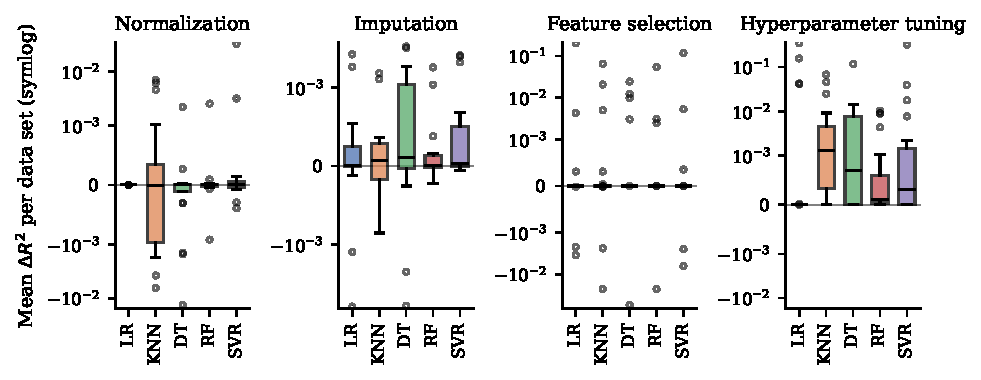
\includegraphics[width=\textwidth]{figuras/fig_overview_box.pdf}
\caption{Distribution of the mean $\Delta R^2$ of each data set, per algorithm and scenario.}
\label{fig:visao-geral}
\legend{Source: The Author. The vertical axis uses a symmetric logarithmic scale, linear between $-10^{-3}$ and $10^{-3}$. Note the different ranges of the panels.}
\end{figure}

The relative ordering of the scenarios is consistent with the nature of the
information that each one leaks (Table~\ref{tab:fontes-vazamento}): the two
scenarios that leak only feature statistics (normalization and imputation)
barely move the estimates, whereas the two scenarios in which the target values
of the test examples influence a decision (which features to keep, which
configuration to report) are the ones that produce substantial inflation.

\section{Normalization}
\label{sec:res-normalizacao}

Table~\ref{tab:alg-normalizacao} details the normalization scenario per
algorithm. No algorithm shows a significant effect (all Holm-adjusted
$p$-values $\geq 0.44$), and the mean $\Delta R^2$ is below $0.002$ for all of
them. Two groups can be distinguished. LR is, in practice, insensitive to the
scenario: 99.2\% of its pairs are exact ties, and the remaining differences are
of the order of $10^{-10}$, i.e., floating-point noise. This is the expected
behavior, since the predictions of an OLS model with intercept do not change under
an affine transformation of the features, whatever the statistics used to define
it. DT and RF are also invariant to monotonic transformations of each feature, so
the differences observed for them (30\% and 43\% of the pairs with a positive
$\Delta R^2$, against 33\% and 51\% with a negative one) cannot result from any
information about the test set; they arise from numerical details, such as the
order in which tied candidate splits are evaluated, and their magnitude can be
taken as the noise floor of the experimental setup.

\begin{table}[htb]
\centering
\caption{Effect of leakage in the normalization scenario, per algorithm.}
\label{tab:alg-normalizacao}
\small
\setlength{\tabcolsep}{3.5pt}
\begin{tabular}{lrrrrrrrr}
\toprule
\textbf{Alg.} & \multicolumn{3}{c}{\textbf{$\Delta R^2$ per data set}} & \textbf{$\Delta$RMSE (\%)} & \textbf{Better} & \textbf{Tie} & \textbf{Worse} & \textbf{$p_{\text{Holm}}$} \\
\cmidrule(lr){2-4}
& Mean & Median & Max & Mean & (\%) & (\%) & (\%) & ($R^2$) \\
\midrule
LR & $3.7\times10^{-12}$ & 0.0000 & $7.8\times10^{-11}$ & 0.00 & 0.8 & 99.2 & 0.0 & 1.000 \\
KNN & 0.0002 & $-7.5\times10^{-6}$ & 0.0070 & -0.01 & 50.8 & 0.0 & 49.2 & 1.000 \\
DT & -0.0007 & 0.0000 & 0.0022 & -0.08 & 30.2 & 36.5 & 33.3 & 0.440 \\
RF & $7.6\times10^{-5}$ & $5.3\times10^{-7}$ & 0.0025 & -0.00 & 42.9 & 6.3 & 50.8 & 1.000 \\
SVR & 0.0017 & $7.4\times10^{-6}$ & 0.0330 & 0.09 & 54.0 & 0.0 & 46.0 & 1.000 \\
\bottomrule
\end{tabular}

\\[2pt]
\footnotesize Source: The Author. Mean, median, and maximum computed over the 21 per-data-set means. Better, Tie, and Worse: percentage of pairs with $\Delta R^2$ above, equal to, or below zero. $p_{\text{Holm}}$: Wilcoxon signed-rank test on the per-data-set means, Holm-adjusted across algorithms.
\end{table}

KNN and SVR, the two scale-sensitive algorithms, never produced ties, as expected:
the standardization parameters estimated on the full data set differ slightly
from those estimated on three quarters of it, and the distances and margins
change accordingly. However, these changes favored the leakage-prone pipeline in
roughly half of the pairs (50.8\% for KNN, 54.0\% for SVR) and penalized it in the
other half, so that the per-data-set means are centered at zero. The largest
effect was observed for SVR on \texttt{542\_pollution}, the third smallest data
set (60 instances), with a mean $\Delta R^2$ of 0.033; apart from it, no
combination exceeded 0.01. In short, fitting the scaler on the full data set
injects variability into the estimate, mostly in very small data sets, but does
not bias it in a consistent direction.

\section{Missing Value Imputation}
\label{sec:res-imputacao}

The imputation scenario comprises 7,560 pairs and is summarized in
Table~\ref{tab:alg-imputacao}. As in normalization, the effects are very small:
no data set--algorithm combination reached a mean $\Delta R^2$ of 0.004, and the
mean over all combinations was 0.0002. Unlike normalization, however, the
direction of the effect is slightly unbalanced in favor of leakage for all
algorithms, with 40\% to 50\% of the pairs improved and 37\% to 43\% worsened.
For SVR this small but systematic shift is statistically significant after the
Holm correction ($p = 0.028$ for $\Delta R^2$ and $p = 0.021$ for $\Delta$RMSE),
with a mean $\Delta R^2$ of 0.0005 and a mean RMSE reduction of 0.11\%.

\begin{table}[htb]
\centering
\caption{Effect of leakage in the imputation scenario, per algorithm (all imputers and missing rates).}
\label{tab:alg-imputacao}
\small
\setlength{\tabcolsep}{3.5pt}
\begin{tabular}{lrrrrrrrr}
\toprule
\textbf{Alg.} & \multicolumn{3}{c}{\textbf{$\Delta R^2$ per data set}} & \textbf{$\Delta$RMSE (\%)} & \textbf{Better} & \textbf{Tie} & \textbf{Worse} & \textbf{$p_{\text{Holm}}$} \\
\cmidrule(lr){2-4}
& Mean & Median & Max & Mean & (\%) & (\%) & (\%) & ($R^2$) \\
\midrule
LR & -0.0001 & $9.8\times10^{-6}$ & 0.0030 & 0.09 & 49.7 & 9.4 & 40.9 & 0.609 \\
KNN & 0.0001 & $6.7\times10^{-5}$ & 0.0016 & 0.04 & 47.0 & 13.2 & 39.8 & 0.747 \\
DT & 0.0002 & 0.0001 & 0.0038 & -0.03 & 40.3 & 22.4 & 37.4 & 0.329 \\
RF & 0.0002 & $2.4\times10^{-6}$ & 0.0019 & 0.02 & 44.6 & 12.5 & 42.9 & 0.747 \\
SVR & 0.0005 & $3.6\times10^{-5}$ & 0.0029 & 0.11 & 48.6 & 9.1 & 42.3 & 0.028 \\
\bottomrule
\end{tabular}

\\[2pt]
\footnotesize Source: The Author. Columns as in Table~\ref{tab:alg-normalizacao}.
\end{table}

The effect depends more on the imputer than on the missing rate.
Table~\ref{tab:alg-imputador} breaks the results down by imputer. The KNN
imputer, which uses the full rows of the neighbors to fill each gap, is the one
that benefits most from having the test instances available: leakage improved the
estimate in 56.7\% of its pairs, against 46.0\% for mean imputation and 35.4\% for
median imputation, and its mean $\Delta R^2$ (0.00036) is about four times that of
the other two imputers (0.00009 and 0.00010). With the KNN imputer, SVR is again
the only algorithm with a significant effect (Holm-adjusted $p = 0.004$). Median
imputation produced many exact ties (28.1\% of its pairs), because the median of
a feature is often the same value whether or not the test fold is included.
Figure~\ref{fig:imputacao-taxa} shows that, contrary to what could be expected,
increasing the missing rate from 5\% to 30\% did not increase the effect: the
Spearman correlation between the missing rate and the mean $\Delta R^2$ of each
configuration is essentially null ($\rho = -0.01$, $p = 0.81$).

\begin{table}[htb]
\centering
\caption{Effect of leakage in the imputation scenario, per imputer and algorithm.}
\label{tab:alg-imputador}
\small
\setlength{\tabcolsep}{3pt}
\begin{tabular}{llrrrrrrrr}
\toprule
\textbf{imputer} & \textbf{Alg.} & \multicolumn{3}{c}{\textbf{$\Delta R^2$ per data set}} & \textbf{$\Delta$RMSE (\%)} & \textbf{Better} & \textbf{Tie} & \textbf{Worse} & \textbf{$p_{\text{Holm}}$} \\
\cmidrule(lr){3-5}
& & Mean & Median & Max & Mean & (\%) & (\%) & (\%) & ($R^2$) \\
\midrule
KNN & LR & -0.0007 & $9.3\times10^{-5}$ & 0.0062 & 0.22 & 60.3 & 1.2 & 38.5 & 0.383 \\
KNN & KNN & 0.0001 & 0.0002 & 0.0030 & 0.09 & 58.3 & 2.2 & 39.5 & 0.473 \\
KNN & DT & 0.0006 & 0.0004 & 0.0115 & -0.07 & 52.4 & 5.6 & 42.1 & 0.383 \\
KNN & RF & 0.0004 & $4.3\times10^{-5}$ & 0.0058 & 0.04 & 55.2 & 1.6 & 43.3 & 0.383 \\
KNN & SVR & 0.0014 & 0.0001 & 0.0098 & 0.28 & 57.1 & 1.2 & 41.7 & 0.004 \\
\midrule
mean & LR & 0.0002 & $1.4\times10^{-7}$ & 0.0024 & 0.02 & 52.0 & 0.2 & 47.8 & 0.786 \\
mean & KNN & 0.0001 & $1.4\times10^{-5}$ & 0.0017 & 0.01 & 47.6 & 8.5 & 43.8 & 1.000 \\
mean & DT & $-1.0\times10^{-5}$ & $1.7\times10^{-5}$ & 0.0015 & 0.02 & 35.1 & 28.8 & 36.1 & 1.000 \\
mean & RF & $4.4\times10^{-6}$ & $-2.7\times10^{-6}$ & 0.0003 & -0.00 & 43.7 & 9.9 & 46.4 & 1.000 \\
mean & SVR & 0.0001 & $1.5\times10^{-5}$ & 0.0024 & -0.00 & 51.6 & 0.0 & 48.4 & 1.000 \\
\midrule
median & LR & 0.0001 & 0.0000 & 0.0015 & 0.02 & 36.7 & 26.8 & 36.5 & 1.000 \\
median & KNN & 0.0001 & 0.0000 & 0.0018 & 0.01 & 35.1 & 28.8 & 36.1 & 1.000 \\
median & DT & 0.0001 & 0.0000 & 0.0029 & -0.05 & 33.3 & 32.7 & 33.9 & 1.000 \\
median & RF & $6.1\times10^{-5}$ & $-3.4\times10^{-7}$ & 0.0017 & 0.00 & 34.9 & 26.0 & 39.1 & 1.000 \\
median & SVR & $4.7\times10^{-5}$ & 0.0000 & 0.0024 & 0.05 & 37.1 & 26.0 & 36.9 & 1.000 \\
\bottomrule
\end{tabular}

\\[2pt]
\footnotesize Source: The Author. Columns as in Table~\ref{tab:alg-normalizacao}; Holm adjustment applied within each imputer.
\end{table}

\begin{figure}[htb]
\centering
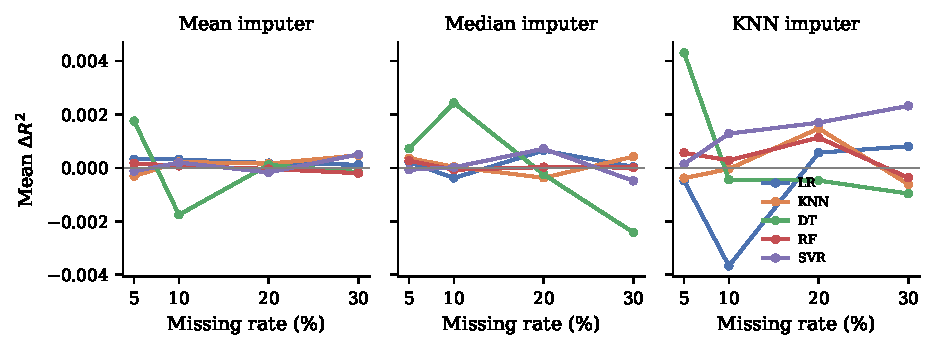
\includegraphics[width=\textwidth]{figuras/fig_imp_rate.pdf}
\caption{Mean $\Delta R^2$ in the imputation scenario as a function of the missing rate, per imputer and algorithm.}
\label{fig:imputacao-taxa}
\legend{Source: The Author}
\end{figure}

Two aspects of the setup help explain the small magnitude of these effects. First,
only about one tenth of the features received missing values
(Section~\ref{sec:met-imputacao}), so most of the information available to the
models was never affected by the imputation step. Second, the imputers leak only
feature statistics, which are estimated almost equally well from 75\% of the data
as from 100\% of it; the additional information carried by the test instances is
therefore marginal. The scenario nevertheless shows that the more an imputer
relies on individual instances rather than on global summaries, as KNN
imputation does, the more it can transfer information between training and test
examples.

\section{Feature Selection}
\label{sec:res-selecao}

The feature selection scenario has the most skewed distribution of effects
(Table~\ref{tab:alg-selecao} and Figure~\ref{fig:heatmap-selecao}). In 93.6\% of
the pairs, the leakage-prone and leakage-free pipelines selected exactly the same
features and therefore produced identical results; of the 420 data
set--algorithm--percentile configurations, 358 were ties in all six repetitions.
When a single feature is kept, which is the case at the 1\% and 5\% levels for
every data set with up to 21 features, and at all levels for the five data sets
with four features, the best-ranked feature is almost always the same whether or
not the test instances are used, and the effect vanishes: 99.0\% and 97.3\% of
the pairs are ties at these two levels. The effect emerges at
10\% and 20\%, when two or more features are kept and the features that compete
for the last positions of the ranking can be swapped by the presence of the test
instances (Figure~\ref{fig:selecao-percentil} and Table~\ref{tab:alg-percentil}
in Appendix~\ref{ap:tabelas}).

\begin{table}[htb]
\centering
\caption{Effect of leakage in the feature selection scenario, per algorithm (all percentiles).}
\label{tab:alg-selecao}
\small
\setlength{\tabcolsep}{3.5pt}
\begin{tabular}{lrrrrrrrr}
\toprule
\textbf{Alg.} & \multicolumn{3}{c}{\textbf{$\Delta R^2$ per data set}} & \textbf{$\Delta$RMSE (\%)} & \textbf{Better} & \textbf{Tie} & \textbf{Worse} & \textbf{$p_{\text{Holm}}$} \\
\cmidrule(lr){2-4}
& Mean & Median & Max & Mean & (\%) & (\%) & (\%) & ($R^2$) \\
\midrule
LR & 0.0095 & 0.0000 & 0.1999 & 0.31 & 3.0 & 95.8 & 1.2 & 1.000 \\
KNN & 0.0032 & 0.0000 & 0.0651 & 0.21 & 8.3 & 84.5 & 7.1 & 1.000 \\
DT & -0.0002 & 0.0000 & 0.0244 & 0.09 & 2.4 & 95.8 & 1.8 & 1.000 \\
RF & 0.0018 & 0.0000 & 0.0542 & 0.14 & 2.4 & 95.8 & 1.8 & 0.995 \\
SVR & 0.0054 & 0.0000 & 0.1172 & 0.26 & 2.6 & 95.8 & 1.6 & 0.582 \\
\bottomrule
\end{tabular}

\\[2pt]
\footnotesize Source: The Author. Columns as in Table~\ref{tab:alg-normalizacao}.
\end{table}

\begin{figure}[htb]
\centering
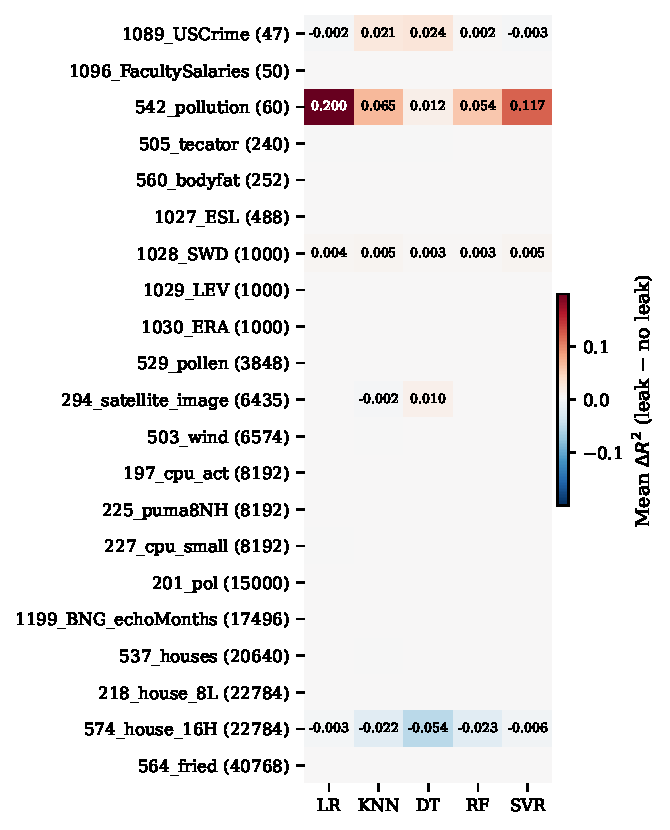
\includegraphics[width=0.75\textwidth]{figuras/fig_heatmap_feature_selection.pdf}
\caption{Mean $\Delta R^2$ per data set and algorithm in the feature selection scenario.}
\label{fig:heatmap-selecao}
\legend{Source: The Author. Data sets are ordered by number of instances (in parentheses); values below 0.0005 in absolute value are omitted.}
\end{figure}

\begin{figure}[htb]
\centering
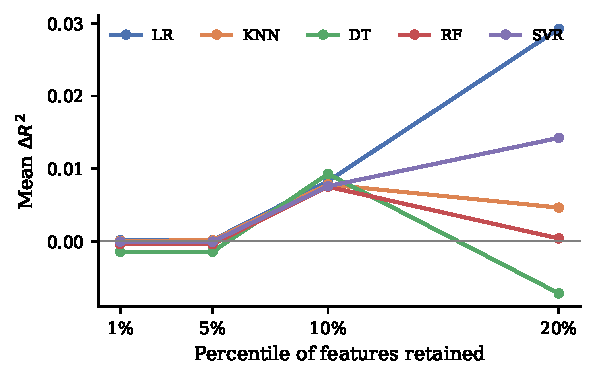
\includegraphics[width=0.62\textwidth]{figuras/fig_fs_perc.pdf}
\caption{Mean $\Delta R^2$ in the feature selection scenario as a function of the percentile of features kept.}
\label{fig:selecao-percentil}
\legend{Source: The Author}
\end{figure}

When the effect appears, it can be large. Table~\ref{tab:top-selecao} lists the
combinations with the largest mean $\Delta R^2$. The data set
\texttt{542\_pollution}, with 60 instances and 15 features, dominates the ranking:
its mean $\Delta R^2$ across percentiles reaches 0.200 for LR, 0.117 for SVR, and
0.065 for KNN. At the 20\% level, LR obtained a leakage-prone $R^2$ of 0.488
against a leakage-free $R^2$ of $-0.130$, i.e., leakage turned a model that is
worse than predicting the mean into one that apparently explains half of the
variance of the target. This is a regression analogue of the selection bias
described by \citeonline{ambroise2002}: with few instances, the features that
correlate best with the target over the full data set include features whose
correlation is partly produced by the test instances themselves, and those
features are then evaluated precisely on those instances. Apart from it, a noticeable positive effect appears only on \texttt{1089\_USCrime}
(47 instances and 13 features, at the 10\% level, with $\Delta R^2$ of 0.097 for
DT and 0.083 for KNN) and on \texttt{1028\_SWD} (at the 20\% level, with
$\Delta R^2$ between 0.012 and 0.021 for all algorithms).

\begin{table}[htb]
\centering
\caption{Data set--algorithm combinations with the largest mean $\Delta R^2$ in the feature selection scenario.}
\label{tab:top-selecao}
\small
\begin{tabular}{llrr}
\toprule
\textbf{Data set} & \textbf{Alg.} & \textbf{$\Delta R^2$} & \textbf{$\Delta$RMSE (\%)} \\
\midrule
542\_pollution & LR & 0.1999 & 6.68 \\
542\_pollution & SVR & 0.1172 & 5.76 \\
542\_pollution & KNN & 0.0651 & 4.48 \\
542\_pollution & RF & 0.0542 & 3.80 \\
1089\_USCrime & DT & 0.0244 & 1.58 \\
1089\_USCrime & KNN & 0.0207 & 1.29 \\
542\_pollution & DT & 0.0124 & 1.61 \\
294\_satellite\_image & DT & 0.0099 & 0.55 \\
\bottomrule
\end{tabular}

\\[2pt]
\footnotesize Source: The Author. Values averaged over percentiles and repetitions.
\end{table}

Feature selection is also the only scenario with a noticeable \emph{negative}
effect. On \texttt{574\_house\_16H}, the features chosen with the full data set
led to a lower $R^2$ than those chosen with the training set alone, with mean
$\Delta R^2$ down to $-0.155$ for DT at the 20\% level. The filter used here ranks
features by their univariate \emph{linear} association with the target, which is
not necessarily the criterion that matters for non-linear models. In large data
sets, where the training set and the full data set produce almost identical
rankings, the occasional swap of a feature near the cutoff is not driven by the
test examples in any meaningful way, and it may favor either pipeline. As a
result, no algorithm shows a significant effect in this scenario (all
Holm-adjusted $p \geq 0.58$), and the Wilcoxon test, which discards ties, is left
with very few informative data sets. The absence of significance should thus be
read as ``rare but potentially severe'' rather than ``harmless''.

\section{Hyperparameter Tuning}
\label{sec:res-tuning}

Hyperparameter tuning is the scenario with the clearest and most consistent
effect (Table~\ref{tab:alg-tuning} and Figure~\ref{fig:heatmap-tuning}). Leakage
improved the performance estimate for all five algorithms, and the effect is
statistically significant for all of them after the Holm correction, both for
$\Delta R^2$ and for $\Delta$RMSE (adjusted $p$-values between $<0.001$ and
$0.028$). The non-nested procedure never produced a substantially worse estimate
than nested CV: only 1.6\% to 8.7\% of the pairs had a negative $\Delta R^2$,
against 15.1\% to 70.6\% with a positive one. In 23 of the 105 data
set--algorithm combinations, leakage improved the estimate in all six
repetitions, against at most one combination in the normalization scenario and
none in the feature selection scenario.

\begin{table}[htb]
\centering
\caption{Effect of leakage in the hyperparameter tuning scenario, per algorithm.}
\label{tab:alg-tuning}
\small
\setlength{\tabcolsep}{3.5pt}
\begin{tabular}{lrrrrrrrr}
\toprule
\textbf{Alg.} & \multicolumn{3}{c}{\textbf{$\Delta R^2$ per data set}} & \textbf{$\Delta$RMSE (\%)} & \textbf{Better} & \textbf{Tie} & \textbf{Worse} & \textbf{$p_{\text{Holm}}$} \\
\cmidrule(lr){2-4}
& Mean & Median & Max & Mean & (\%) & (\%) & (\%) & ($R^2$) \\
\midrule
LR & 0.0281 & 0.0000 & 0.3489 & 4.61 & 15.1 & 83.3 & 1.6 & 0.028 \\
KNN & 0.0083 & 0.0013 & 0.0683 & 1.11 & 70.6 & 22.2 & 7.1 & $<$0.001 \\
DT & 0.0089 & 0.0007 & 0.1181 & 1.17 & 38.9 & 52.4 & 8.7 & 0.004 \\
RF & 0.0017 & 0.0001 & 0.0103 & 0.34 & 59.5 & 31.7 & 8.7 & $<$0.001 \\
SVR & 0.0188 & 0.0003 & 0.3212 & 2.18 & 38.9 & 58.7 & 2.4 & 0.004 \\
\bottomrule
\end{tabular}

\\[2pt]
\footnotesize Source: The Author. Columns as in Table~\ref{tab:alg-normalizacao}.
\end{table}

\begin{figure}[htb]
\centering
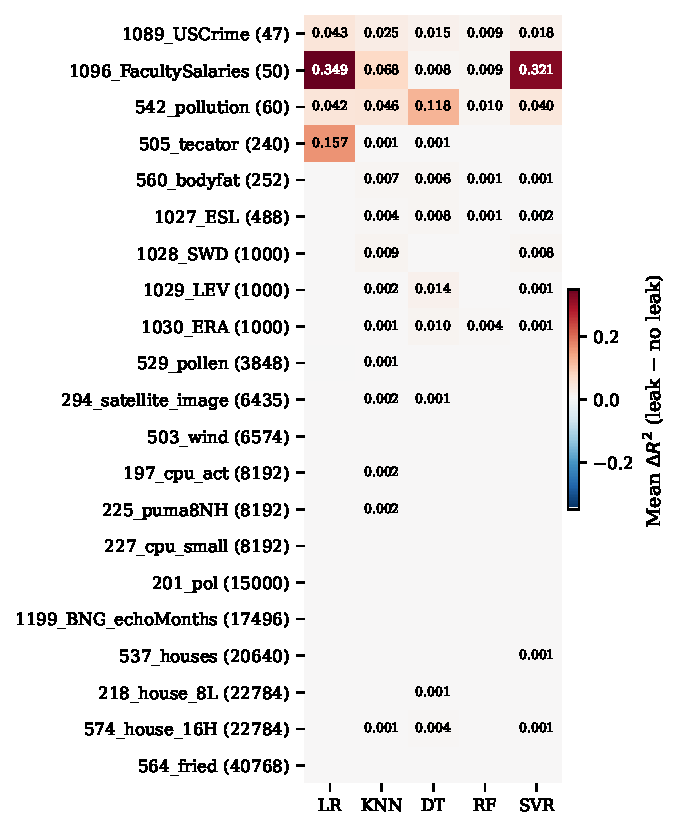
\includegraphics[width=0.75\textwidth]{figuras/fig_heatmap_tuning.pdf}
\caption{Mean $\Delta R^2$ per data set and algorithm in the hyperparameter tuning scenario.}
\label{fig:heatmap-tuning}
\legend{Source: The Author. Data sets are ordered by number of instances (in parentheses); values below 0.0005 in absolute value are omitted.}
\end{figure}

The algorithms differ in how often and how strongly they are affected. KNN and
RF are affected most frequently, with a positive mean $\Delta R^2$ in 19 of the
21 data sets and 70.6\% and 59.5\% of the pairs improved, respectively; for these
algorithms, several configurations in the grid have similar performance and
noise decides which one looks best, so that reporting the best CV score
systematically picks up a small positive bias. The magnitude of that bias, however,
is moderate (mean $\Delta R^2$ of 0.0083 for KNN and 0.0017 for RF). LR shows the
opposite pattern: 83.3\% of its pairs are exact ties, because the four
configurations of its grid frequently lead the inner and outer searches to the
same choice, in which case nested and non-nested CV report exactly the same
score. When the choice is not stable, the effect is very large, and LR has the
highest mean $\Delta R^2$ (0.028) and $\Delta$RMSE (4.6\%) of all algorithms.

Table~\ref{tab:top-tuning} lists the most affected combinations. On
\texttt{1096\_FacultySalaries} (50 instances), the non-nested estimate of $R^2$
was 0.826 for LR and 0.827 for SVR, while nested CV estimated 0.478 and 0.506,
respectively; this corresponds to differences of 0.349 and 0.321 in $R^2$ and to
RMSE reductions of about one third. On \texttt{505\_tecator}, which has more
features than half of its number of instances, LR reached an $R^2$ of 0.985 with
leakage against 0.828 without it, and the RMSE was underestimated by 54\%. Since
the leakage-prone pipeline reports, for each metric, the best value over the
grid, part of this optimism also comes from the possibility of choosing a
different configuration for each metric, a freedom that a properly validated
pipeline does not have.

\begin{table}[htb]
\centering
\caption{Data set--algorithm combinations with the largest mean $\Delta R^2$ in the hyperparameter tuning scenario.}
\label{tab:top-tuning}
\small
\begin{tabular}{llrr}
\toprule
\textbf{Data set} & \textbf{Alg.} & \textbf{$\Delta R^2$} & \textbf{$\Delta$RMSE (\%)} \\
\midrule
1096\_FacultySalaries & LR & 0.3489 & 34.07 \\
1096\_FacultySalaries & SVR & 0.3212 & 33.23 \\
505\_tecator & LR & 0.1573 & 54.18 \\
542\_pollution & DT & 0.1181 & 5.66 \\
1096\_FacultySalaries & KNN & 0.0683 & 8.41 \\
542\_pollution & KNN & 0.0463 & 2.89 \\
1089\_USCrime & LR & 0.0427 & 5.10 \\
542\_pollution & LR & 0.0417 & 3.52 \\
\bottomrule
\end{tabular}

\\[2pt]
\footnotesize Source: The Author. Values averaged over repetitions.
\end{table}

\section{Sensitivity of the Algorithms}
\label{sec:res-algoritmos}

To compare the algorithms, the Friedman test was applied, within each scenario,
to the per-data-set mean $\Delta R^2$ of the five algorithms. A significant
difference between algorithms was found only for hyperparameter tuning
($\chi^2_F = 17.73$, $p = 0.001$). In this scenario, the average ranks
(1 = most affected) were 1.90 for KNN, 2.83 for DT, 3.26 for RF and SVR, and 3.74
for LR, confirming that KNN is the algorithm most consistently inflated by
non-nested tuning, even though LR and SVR present the most extreme individual
cases. In the feature selection scenario, the test approached significance
($\chi^2_F = 8.16$, $p = 0.086$), with SVR ranked first (2.38); in normalization
($p = 0.41$) and imputation ($p = 0.45$), the algorithms are indistinguishable.

Taken together, the results suggest that the sensitivity of an algorithm depends
on the mechanism of leakage rather than being an intrinsic property of the
algorithm. Scale-sensitive algorithms (KNN and SVR) are the only ones that can
react to normalization leakage at all, but the reaction is noisy and not biased.
SVR is the only algorithm with a significant effect in the imputation scenario,
and it appears among the most affected combinations in feature selection and
tuning, which makes it the algorithm that was most often affected across
scenarios. Tree-based models are the least affected overall: they are insensitive
to scaling, and RF, in particular, presented the smallest maximum effects in
tuning (0.010) among all algorithms. LR is either completely unaffected or
strongly affected, depending on whether the leakage mechanism changes the
information available to it.

\section{Influence of Data Set Characteristics}
\label{sec:res-datasets}

Figure~\ref{fig:tamanho} relates the mean $\Delta R^2$ of each data
set--algorithm combination to the number of instances of the data set. The
largest effects of all four scenarios concentrate on the left of the plots. The
six data sets with fewer than 1,000 instances account for most of the inflation:
in the tuning scenario, their mean $\Delta R^2$ is 0.044, against 0.001 for the
15 larger data sets, and in feature selection it is 0.016, against $-0.001$. Even
in normalization and imputation, the mean absolute $\Delta R^2$ of the small data
sets is about six to nine times that of the large ones (0.0039 vs.\ 0.0005 and
0.0066 vs.\ 0.0011, respectively), which indicates that leakage also increases
the variability of the estimates when data are scarce.

\begin{figure}[htb]
\centering
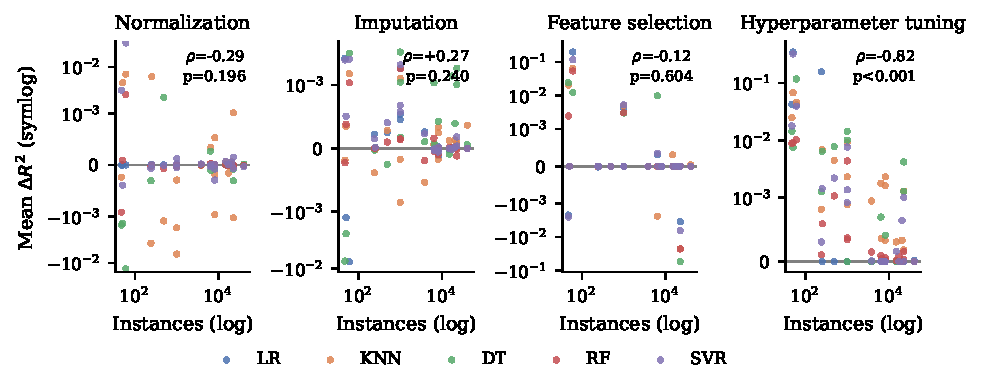
\includegraphics[width=\textwidth]{figuras/fig_delta_vs_size.pdf}
\caption{Mean $\Delta R^2$ per data set and algorithm versus the number of instances of the data set.}
\label{fig:tamanho}
\legend{Source: The Author. Spearman $\rho$ computed between the number of instances and the mean $\Delta R^2$ of each data set (averaged over algorithms). Vertical axis in symmetric logarithmic scale.}
\end{figure}

The Spearman correlations confirm this relation for hyperparameter tuning: the
per-data-set mean $\Delta R^2$ is strongly and negatively correlated with the
number of instances ($\rho = -0.82$, $p < 0.001$) and positively correlated with
the features-to-instances ratio ($\rho = 0.82$, $p < 0.001$), whereas the number
of features alone shows no association ($\rho = -0.06$, $p = 0.80$). For the other
three scenarios, none of the correlations is significant ($\lvert\rho\rvert \leq
0.29$, $p \geq 0.20$). In the feature selection scenario, the lack of
correlation reflects the fact that the effect depends on a combination of
conditions, namely few instances \emph{and} enough features for the selection to
be unstable, which only a handful of data sets satisfy.

These findings have a simple interpretation. Both CV estimates and univariate
feature rankings are noisier when they are computed from few instances. Leakage
lets the pipeline choose, among several noisy alternatives, the one that happens
to fit the test examples best, and the more noise there is, the larger the gain
of that choice. In large data sets, all alternatives are estimated accurately,
the choice made with the test examples coincides with the choice made without
them, and the leakage becomes inconsequential.

\section{Discussion}
\label{sec:res-discussao}

\subsection{Answers to the Research Questions}

\textbf{RQ1 -- Does leakage inflate performance estimates?} It depends on the
step. Leakage in hyperparameter tuning inflated the estimates of all five
algorithms significantly. Leakage in feature selection inflated them strongly in
a few small data sets but left most configurations unchanged. Leakage in
normalization and imputation produced changes close to the noise floor of the
experiments, with a small but significant bias only for SVR combined with
imputation.

\textbf{RQ2 -- Which step produces the largest distortions?} Hyperparameter
tuning, both in frequency and in average magnitude, followed by feature selection,
which produced comparable maximum effects but much less often. Normalization and
imputation produced effects one to two orders of magnitude smaller. The ranking
follows the type of information that leaks: steps that leak information about the
target are far more harmful than steps that leak only feature statistics.

\textbf{RQ3 -- Are some algorithms more sensitive?} Only in the tuning scenario
did the algorithms differ significantly. KNN was the most consistently affected
algorithm in that scenario, while LR and SVR presented the largest individual
distortions. Across scenarios, SVR was the algorithm that was most often among the
affected ones, and tree-based models, especially RF, were the least affected.

\textbf{RQ4 -- Do data set characteristics matter?} Yes. The number of instances
was the most relevant factor: the largest distortions occurred in data sets with
fewer than 1,000 instances, and, for tuning, the effect was strongly correlated
with the number of instances and with the features-to-instances ratio.

\subsection{Comparison with Classification}

\citeonline{becker2023} reported, for classification, that feature selection and
hyperparameter tuning were the steps with the largest effects and that SVM was
more susceptible than other algorithms. The present results agree on the first
point: in regression as well, the steps that use the target are the dangerous
ones. They also agree that the support vector family is among the most sensitive
algorithms. The main difference concerns the relative weight of feature
selection, which in this study produced severe distortions only in a few data
sets. Part of this difference can be attributed to the design of the
experiments, as discussed below, and part to the continuous nature of the
target. Since $R^2$ and RMSE are continuous functions of every prediction, a
small change in the pipeline always produces a small change in the metric,
whereas accuracy-like metrics change in discrete steps; at the same time, the
absence of an upper bound for the error metrics means that, in small data sets,
a single leaky decision may change the RMSE by tens of percent, as observed for
\texttt{1096\_FacultySalaries} and \texttt{505\_tecator}.

\subsection{Threats to Validity}

Some decisions of the experimental design limit the generality of the results.
Concerning \emph{internal validity}, the imputation scenario introduced missing
values in only about one tenth of the features, under a single MAR mechanism;
higher proportions of incomplete features or MNAR mechanisms could produce larger
effects. In addition, the random choice of which features receive missing values
is not controlled by the fixed seed used to generate the mask, so this choice may
differ between executions, although it is identical for the two pipelines of each
pair. The feature selection scenario used small percentiles that, in data sets
with few features, collapse into a single selected feature, which reduces the
number of informative configurations; and it used a hold-out protocol, whereas the
other scenarios used CV. In the normalization, imputation, and feature selection
scenarios, SVR was trained with a linear solver, so the conclusions about SVR in
these scenarios refer to linear SVR.

Concerning \emph{external validity}, the 21 data sets, although diverse, are a
small sample of regression problems, and only six of them have fewer than 1,000
instances, which is precisely the range where the effects appear. A larger number
of small data sets would allow the relation between size and leakage to be
characterized more precisely. Finally, concerning \emph{conclusion validity}, the
Wilcoxon tests were performed with 21 data sets per algorithm, and ties are
discarded by the test, which reduces its power in scenarios such as feature
selection; the absence of significance in those scenarios should not be
interpreted as evidence that leakage is harmless.
